% !BIB TS-program = bibtex

%-----------------------------------------------------------------------------
%
% Conference SASO - https://saso2017.telecom-paristech.fr/
% Page limit: 10 pages 
% Submission deadline: 
%			Abstract: May 8st
%			Full paper: May 24th
% Notification: June 30th
% Revisions: July 10th 
%
%-----------------------------------------------------------------------------

\documentclass[draft]{llncs}


%---- PACKAGES
%\usepackage{todonotes}
\usepackage{amssymb}
\usepackage{hyperref}
\usepackage[plain]{fancyref}
\usepackage{ifdraft}
%\usepackage{subcaption}
\let\labelindent\relax
\usepackage[inline]{enumitem}
\usepackage{xcolor}
\usepackage[final]{graphicx}
\usepackage{xspace}
\usepackage[final]{listings}
\usepackage{acronym}
\usepackage{url}
\usepackage{amsmath}
\usepackage{amssymb}
\usepackage[square,numbers,sectionbib]{natbib}
\bibliographystyle{abbrvnat}

\usepackage{etoolbox}
\makeatletter
\patchcmd{\@makecaption}
  {\scshape}
  {}
  {}
  {}
\patchcmd{\@makecaption}
  {\\}
  {.\ }
  {}
  {}
\makeatother

%\let\refsection\relax
%\usepackage
%  [backend=biber,
%   style=trad-abbrv,
%   maxnames=5,
%   firstinits=true,
%   hyperref=true,
%   natbib=true,
%   url=false,
%   doi=false,
%   defernumbers]{biblatex}
%
%
%----[ Biber ]----
%\addbibresource[datatype=bibtex]{local.bib}
%\addbibresource[datatype=bibtex]{bib/general.bib}
%\addbibresource[datatype=bibtex]{bib/compsci.bib}
%\addbibresource[datatype=bibtex]{bib/learning.bib}
%\nocite{*}
%
%\newbibmacro{name:newformat}{%
%    \printnames{authors}
%%   \textbf{\namepartfamily}  % #1->\namepartfamily, #2->\namepartfamilyi
%%   \textbf{\namepartgiven}   % #3->\namepartgiven,  #4->\namepartgiveni
%%   [prefix: \namepartprefix] % #5->\namepartprefix, #6->\namepartprefixi
%%   [suffix: \namepartsuffix] % #7->\namepartsuffix, #8->\namepartsuffixi
%}
%
%\DeclareNameFormat{newformat}{%
%  \usebibmacro{name:newformat}{\textbf{#1}}{\textbf{#3}}{#5}{#7}%
%  \usebibmacro{name:andothers}%
%%  \nameparts{#1}% split the name data, will not be necessary in future versions
%%  \usebibmacro{name:newformat}%
%%  \usebibmacro{name:andothers}%
%}
%
%\AtEveryBibitem
%{
%   \clearlist{address}
%   \clearfield{date}
%   \clearfield{doi}
%   \clearfield{eprint}
%   \clearfield{isbn}
%   \clearfield{issn}
%   \clearfield{month}
%   \clearfield{note}
%%   \clearfield{pages}
%   \clearlist{location}
%%   \clearfield{series}
%   \clearfield{url}
%   \clearname{editor}
%   \ifentrytype{inproceedings}
%     {\clearfield{day}
%      \clearfield{month}
%      \clearfield{volume}}{}
%}
%
%\DeclareFieldFormat*{title}{\textsl{#1}\isdot}
%\DeclareFieldFormat*{journaltitle}{#1}
%\DeclareFieldFormat*{booktitle}{#1}
%
%\renewbibmacro{in:}{} % supress 'In: ' form
%
%\DeclareSourcemap
% {\maps[datatype=bibtex,overwrite]
%   {% Tag entries (through keywords)
%    \map
%      {\step[fieldsource=booktitle,
%       match=\regexp{[Pp]roceedings}, replace={Proc.}]}
%        \map
%      {\step[fieldsource=booktitle,
%       match=\regexp{[Ii]nternational\s+[Cc]onference}, replace={Intl. Conf.}]}
%    \map
%      {\step[fieldsource=journal,
%       match=\regexp{[Jj]ournal}, replace={Jour.}]}
%    \map
%      {\step[fieldsource=journal,
%       match=\regexp{[Tt]ransactions}, replace={Trans.}]}
%    \map
%      {\step[fieldsource=booktitle,
%       match=\regexp{[Pp]roceedings\s+of\s+the.+[Ee]uropean\s+[Cc]onference\s+in}, replace={European Conf. in}]}
%    \map
%      {\step[fieldsource=booktitle,
%       match=\regexp{In\s+[Pp]roceedings\s+of\s+the.+[Ss]ymposium\s+on}, replace={Symp. on}]}
%    \map
%      {\step[fieldsource=booktitle,
%       match=\regexp{[Pp]roceedings\s+of\s+the.+[Ii]nternational\s+[Cc]onference\s+on}, replace={Intl. Conf. on}]}
%    \map
%      {\step[fieldsource=booktitle,
%       match=\regexp{[Pp]roceedings\s+of\s+the.+[Ii]nternational\s+[Ww]orkshop\s+on}, replace={Intl. Workshop on}]}}}
%

%color
\definecolor{OliveGreen}{rgb}{0,0.6,0.3}

%References
%% Listings
\def\fref{\Fref} % treat all \frefs as \Frefs
\renewcommand{\lstlistingname}{Snippet}
\newcommand*{\fancyreflstlabelprefix}{lst}
\newcommand*{\Freflstname}{\lstlistingname}
\newcommand*{\freflstname}{\MakeLowercase{\lstlistingname}}
\Frefformat{vario}{\fancyreflstlabelprefix}%
  {\Freflstname\fancyrefdefaultspacing#1#3}
\frefformat{vario}{\fancyreflstlabelprefix}%
  {\freflstname\fancyrefdefaultspacing#1#3}
\Frefformat{plain}{\fancyreflstlabelprefix}%
  {\Freflstname\fancyrefdefaultspacing#1}
\frefformat{plain}{\fancyreflstlabelprefix}%
  {\freflstname\fancyrefdefaultspacing#1}

\renewcommand{\tablename}{Table}  
  
% ln delimiter
\newcommand*{\fancyreflnlabelprefix}{ln}
\newcommand*{\Freflnname}{Line}
\newcommand*{\freflnname}{\MakeLowercase{\Freflnname}}
\Frefformat{vario}{\fancyreflnlabelprefix}%
  {\Freflnname\fancyrefdefaultspacing#1#3}
\frefformat{vario}{\fancyreflnlabelprefix}%
  {\freflnname\fancyrefdefaultspacing#1#3}
\Frefformat{plain}{\fancyreflnlabelprefix}%
  {\Freflnname\fancyrefdefaultspacing#1}
\frefformat{plain}{\fancyreflnlabelprefix}%
  {\freflnname\fancyrefdefaultspacing#1}    


%JavaScript definition
\lstdefinelanguage{JavaScript}{
keywords={typeof, new, true, false, catch, function, return, null, catch, switch, var, if, in, for, while, do, else, case, break, throw, this, instanceof},
keywordstyle=\color{purple}\bfseries,
ndkeywords={},
ndkeywordstyle=\color{blue}\bfseries,
identifierstyle=\color{black},
sensitive=false,
comment=[l]{//},
morecomment=[s]{/*}{*/},
commentstyle=\color{OliveGreen}\ttfamily,
stringstyle=\color{OliveGreen}\ttfamily,
morestring=[b]',
morestring=[b]"
}

\lstset{%
  basicstyle=\small\ttfamily,
  aboveskip=0\baselineskip,
  belowskip=0\baselineskip,
  commentstyle=\color{gray}\footnotesize\ttfamily\itshape,
  prebreak= ,
  numberblanklines=false,
  breaklines,
  numberstyle=\tiny\color{gray}, 
  numbersep=0pt,
  escapechar=`}

\lstdefinestyle{floating}{%
  frame=none,
  float=htb,
  captionpos=b,
  aboveskip=0pt,
  belowskip=0pt
}

% context traits listings
\lstdefinestyle{ctxtraits}
 {language=JavaScript,
  frame=lines,
  showstringspaces=false,
  keywordstyle=\tt\bf,
  tabsize=3,
  style=floating,
  morekeywords={Trait, cop, proceed, Context, activate, deactivate, adapt, addObjectPolicy, manager}
}

%context traits environment    
\lstnewenvironment{ctxtraits}[1][]
 {\lstset{style=ctxtraits,#1}}{}  


 % Context Traits in line source-code
\newcommand{\scode}[1]{\textrm{\texttt{#1}}}
\def\scode{\lstinline[style=ctxtraits]}

%----[ Commands ]---
%Latins
\newcommand{\eg}{\emph{e.g.,}\xspace}
\newcommand{\ie}{\emph{i.e.,}\xspace}
\newcommand{\cf}{\emph{cf.}\xspace}

\newcommand{\ctx}[1]{\texttt{\textsc{#1}}}


%comments
% xcolor
\definecolor{author}{rgb}{.5, .5, .5}
\definecolor{comment}{rgb}{.1, .0, .9}
\definecolor{note}{rgb}{.9, .4, .0}
\definecolor{idea}{rgb}{.1, .7, .0}
\definecolor{missing}{rgb}{.9, .1, .0}


\newcommand{\authorcomment}[3][comment]
  {\ifdraft{\noindent
      \fbox{\footnotesize\textcolor{author}{\textsc{#2}}}
      \textcolor{#1}{\textsl{#3}}}{}}

%% Space-squeezing stuff

\let\origSubsubsection\subsubsection
\renewcommand*{\subsubsection}[1]%
  {\vspace{-1em}\origSubsubsection{#1}}

\makeatletter

% Squeeze figures
\let\orig@figure\figure
\renewcommand*{\figure}[1][]{\orig@figure[#1]\vspace{-0.6em}} % before
\let\orig@endfigure\endfigure
\renewcommand*{\endfigure}{\vspace{-0.7ex}\orig@endfigure} % after

% Squeeze tables
\let\orig@table\table
\renewcommand*{\table}{\orig@table\vspace{-1em}} % before
\let\orig@endtable\endtable
\renewcommand*{\endtable}{\vspace{-1ex}\orig@endtable} % after

% Squeeze snippets
\let\orig@lstlisting\lstlisting
\renewcommand*{\lstlisting}{\orig@lstlisting\vspace{-2em}} % before
\let\orig@endlstlisting\endlstlisting
\renewcommand*{\endlstlisting}{\vspace{-3ex}\orig@endlstlisting} % after



% Squeeze captions
\usepackage{caption}
\captionsetup[figure]{aboveskip=1ex,belowskip=-1em}
\captionsetup[table]{aboveskip=1ex,belowskip=-1em}

% Squeeze section titles
%\let\orig@section\section
%\renewcommand*{\section}[1]{\orig@section{#1}\vspace{-.2ex}}

% Squeeze subsections
\let\orig@subsection\subsection
\renewcommand*{\subsection}[1]{\orig@subsection{#1}\vspace{-.5ex}}

\makeatother


\acrodef{AST}{Abstract Syntax Tree}
\acrodef{COP}{Context-oriented Programming}
\acrodef{MAS}{Multi-Agent System}
\acrodef{RL}{Reinforcement Learning}
\acrodef{ROP}{Role-oriented Programming}
\acrodef{SOC}{Service-oriented Computing}




\begin{document}


% --- End of Author Metadata ---

\title{CollabIDE}
\subtitle{A collaborative IDE for dynamic multi-versioning and variant management}
%Gearing development of variability systems through self-adaptation

%
% You need the command \numberofauthors to handle the 'placement
% and alignment' of the authors beneath the title.
%
% For aesthetic reasons, we recommend 'three authors at a time'
% i.e. three 'name/affiliation blocks' be placed beneath the title.
%
% NOTE: You are NOT restricted in how many 'rows' of
% "name/affiliations" may appear. We just ask that you restrict
% the number of 'columns' to three.
%
% Because of the available 'opening page real-estate'
% we ask you to refrain from putting more than six authors
% (two rows with three columns) beneath the article title.
% More than six makes the first-page appear very cluttered indeed.
%
% Use the \alignauthor commands to handle the names
% and affiliations for an 'aesthetic maximum' of six authors.
% Add names, affiliations, addresses for
% the seventh etc. author(s) as the argument for the
% \additionalauthors command.
% These 'additional authors' will be output/set for you
% without further effort on your part as the last section in
% the body of your article BEFORE References or any Appendices.


\author{
Santiago Beltr\'{a}n \and Nicol\'{a}s Cardozo
}
\institute{
Systems and Computing Engineering Department\\
Universidad de los Andes -  
Bogot\'a, Colombia\\
\email{\{s.beltran10, n.cardozo\}@uniandes.edu.co}
}



% Just remember to make sure that the TOTAL number of authors
% is the number that will appear on the first page PLUS the
% number that will appear in the \additionalauthors section.

\maketitle

% $  Id: conclusion.tex  $
% !TEX root = main.tex

\begin{abstract}
Current practices in software development are anchored in the use of versioning control systems to manage the development progress, or drive the release process. Despite the benefits, using such systems requires developers to interrupt their workflow in order to interact with the versioning system, affecting their productivity. 

\end{abstract}


\endinput
versiones, la enorme cantidad de conveniencias que estos sistemas traen al proyecto hacen que se vuelvan indispensables para el equipo. A pesar de los beneficios que estos sistemas traen, su uso hace que los desarrolladores incurran en un costo adicional de productividad, este costo se origina en la necesidad de los desarrolladores de interrumpir su flujo de trabajo de codificación para llevar a cabo operaciones relacionadas al control de versiones que en algunos casos pueden ser demoradas. En este trabajo presentamos a CollabIDE, un ambiente integrado de desarrollo online que facilita el desarrollo colaborativo alrededor de un proyecto de software y cuyas características están diseñadas para reducir el tiempo que un desarrollador debe invertir en realizar operaciones de versionamiento. A través de un experimento demostramos la efectividad de CollabIDE en reducir el overhead de los sistemas de control de versiones en un modelo de desarrollo dsitribuido y uno modelo de desarrollo basado en líneas de producto.  

\keywords{
Collaborative development, Version control, Software variability, Context-oriented programming 
}
%
% The code below should be generated by the tool at
% http://dl.acm.org/ccs.cfm
% Please copy and paste the code instead of the example below. 
%
%\begin{IEEEkeywords}
%Context-oriented programming, Collaborative development
%\end{IEEEkeywords}


%
%

%%
\section{Introduction}
\label{sec:introduction}

Version Control Systems (VSC) have become a fundamental part in software development projects. 
Among the benefits of using version control are having the change history of every file for traceability 
and branching and merging for working on independent streams of changes. With version control, 
development teams see an improvement in efficiency and reduce the risk of losing progress in the 
project.
One software development model that has gained substantial popularity in recent years is the 
Distributed Software Development model (DSD). This model brings various advantages to 
development teams like costs reduction, increased productivity and ease of finding human talent 
across the globe. In this model team members are geographically distributed and must collaborate 
remotely. Mechanisms like commiting, pushing and merging help team members solve synchronization 
and coordination problems that arise in DSD. However, these mechanisms introduce an overhead 
problem that stems from the interruption in the coding workflow the developers make when they 
perform an action related to version control. Initially this overhead problem may not have much impact 
on the project but in the long term, the productivity of the team can be negatively affected.
Another software development model that has acquired popularity due to the competitive advantages 
it brings to development teams is the \ac{SPL} development model~\cite{pohl+05sple}. Like the DSD 
model, the SPL also suffers from an overhead problem. In this case the problem is caused by the initial 
coding and configuration that must be done at the beginning of a project.
With CollabIDE, we aim to solve the overhead problems that exists in these development models with 
features that aim to reduce the time developers must spend doing actions related to version control or 
setting up a project that uses \acp{SPL}.




\endinput
% $  Id: collabide.tex  $
% !TEX root = main.tex

%%
\section{CollabIDE}
\label{sec:collab-ide}

CollabIDE is a cloud-based integrated development environment presenting collaboration facilities 
distributed development teams working on a software project. CollabIDE has three key features which 
help to reduce the overhead of managing versions or product variants. These features are:
\begin{enumerate*}[label=(\arabic*)] 
\item version management, 
\item product variant management, and 
\item concurrent development.
\end{enumerate*}

%%
\subsection{Version Management}
\label{sec:vcs}
Software products evolve over time~\cite{lehman02}. Rather than releasing a fully working product at 
once, developers implement products incrementally. Each product increment focuses on a single 
feature or part of the functionality at a time. Each of these features marks a new \emph{version} of the 
system, moving forward linearly in time. Defining and synchronizing between these pieces of 
functionality must be carried out multiple times in a project's lifespan. In the long-term, this process 
has a lasting impact in the productivity.

CollabIDE takes the association between a feature's development, and program versions to an 
extreme. In CollabIDE, every code modification (regardless of its size) is marked as a new product 
increment. Furthermore, instead of asking developers to continuously create and manage product 
versions, CollabIDE automatically generates versions for each code increment. These increments are 
identified by a set of variables relevant to the project development. For example, relevant information 
to generate versions may include the developer's name, or the time of the day. Additionally, if 
developers want to create their own versions, it is posible to do so simply by giving them a name in 
the versions pane of the interface. \fref{fig:versions} shows the way product versions are 
managed in the CollabIDE. 

A differentiating feature of CollabIDE is that versions are live. That is, every time a new version is 
created by any of the developers, this is made available to all other developers immediately. 
As a consequence, versioning conflicts become nonexistent as all developers see a sing (and most 
updated) version of the code at all times. Moreover, switching between versions, developers have an 
immediate view of the complete state of the code at the moment the version was created or edited. 

\begin{figure}[tbp]
  \centering
  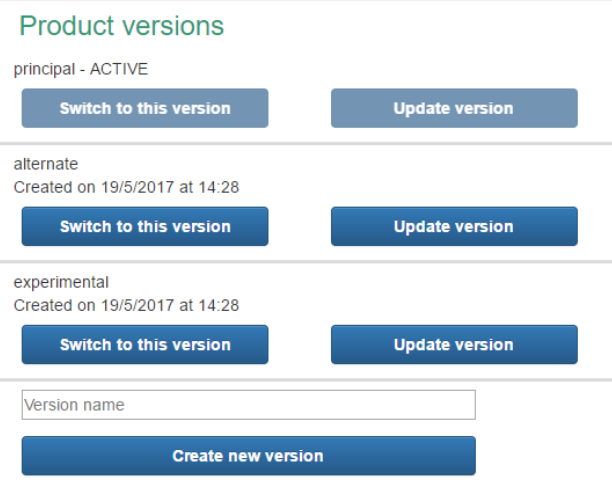
\includegraphics[width=0.7\textwidth]{img/fig4-collabIDEVersionManagement}
  \caption{Version visualization and management in CollabIDE}
  \label{fig:versions}
\end{figure}

The facilities for version management in CollabIDE help reduce the long-term impact of creating, 
updating, and synchronizing product versions, as these processes occur autonomously upon simple 
interactions.

%%
\subsection{Product Variant Management}
\label{sec:product-variant}
In \ac{SPL} development product variants are managed through variability models, describing the 
different components of the product, and the different options for each of these 
components~\cite{pohl05}. A product variant consists of the composition of a base product with 
different features, usually specialized for each costumer or purpose. This process requires developers 
to define beforehand both, the base product, and the variations points (\ie those features that can be 
interchanged with other features). This process is time consuming for the project setup, and fixed in 
the points where variations may take place.

CollabIDE takes advantage of its \ac{VCS} to enable a more flexible product variation model. Product 
variants are defined by the composition of the different versions available in the system. These 
versions may be chosen based on the time of their creation (as explained in the previous section), or 
taking into account the contributions made by specific developers. The composition takes place 
behind the scene using \ac{COP} facilities for dynamic software composition (\cf 
\fref{sec:implementation}).

\fref{fig:contribution} shows the panel in the CollabIDE interface to select the different variants, in this 
case according to developers' contributions. Selecting one of the contributions renders the associated 
code as part of the interface, and composes the variant with the currently working code. From a 
product variant point of view, this feature eases the process of building new variants from existing 
fragments of code, effectively reducing the overhead derived from executing initial configuration 
processes.

\begin{figure}[htbp]
  \centering
  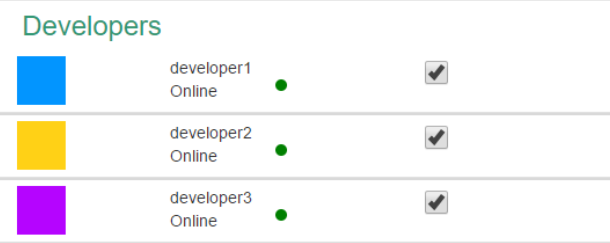
\includegraphics[width=0.7\textwidth]{img/fig3-collabIDEContributionManagement}
  \caption{Product composition through contribution selection}
  \label{fig:contribution}
\end{figure}


%%
\subsection{Concurrent Development}

CollabIDE offers a feature for concurrent development. Taking advantage of the \ac{VCS}, developers 
are able to work concurrently on the same code base, having immediate feedback about the 
contributions of other developers.
Developers' code is differentiated by highlighting, in a unique color, the code contributed by each 
developer, as shown in \fref{fig:layers}. First, colored code, offers a first-hand view about the 
contributions of each team member, increasing awareness  about code owners, and coordination to 
develop or fix code increments. Second, code highlighting is used as a means to identify feature a 
developer has worked on, enabling the composition of specific product variants by selecting the work 
of developers associated to specific features. 

\begin{figure}[htbp]
  \centering
  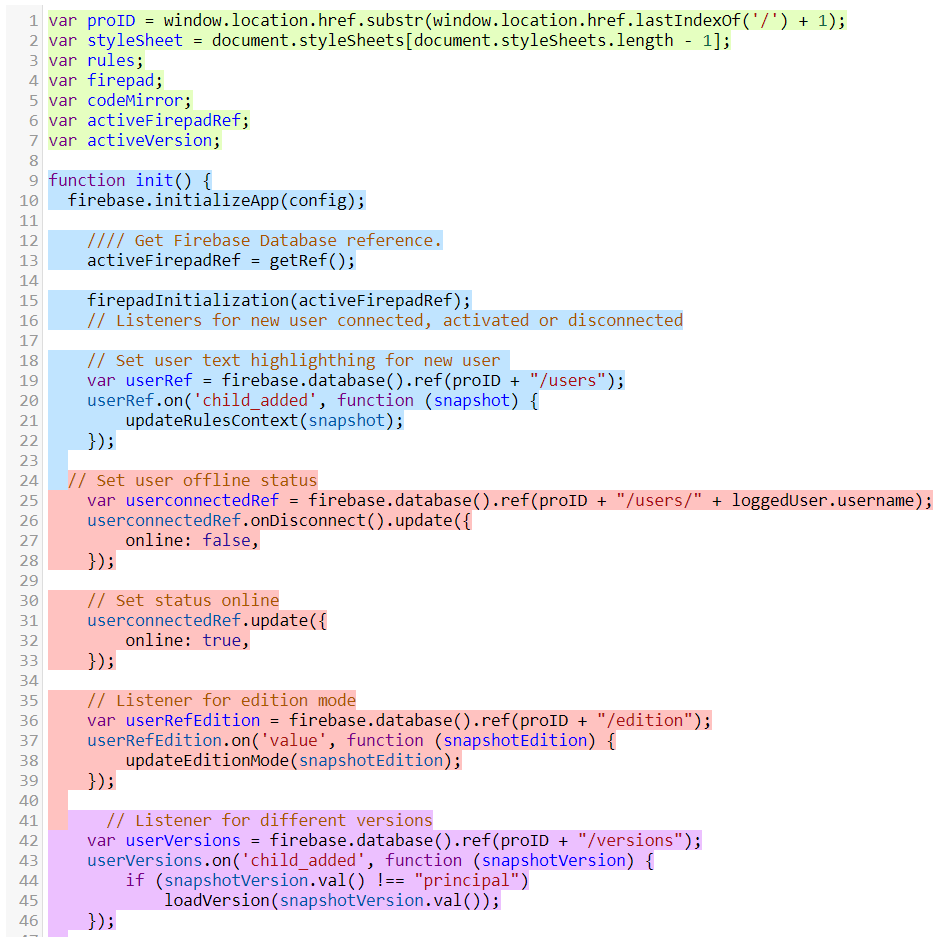
\includegraphics[width=0.7\textwidth]{img/fig2-collabIDEConcurrentProgramming}
  \caption{First-hand view of developers' contributions}
  \label{fig:layers}
\end{figure}


%%
\subsection{Implementation}
\label{sec:implementation}

The implementation of CollabIDE reconciles \ac{COP} with developing software systems integrated as part of a cloud-based platform.

%%%%
\subsubsection{\ac{COP} in a Nutshell}
The base of CollabIDE is \acf{COP}. \ac{COP} is a programming paradigm designed for the dynamic adaptation of software systems based on context information gathered from the system's surrounding execution environment~\cite{salvaneschi+12survey}. \ac{COP} consists of three main abstractions: \emph{Contexts}, \emph{Behavioral adaptations}, \emph{Adaptation activation}.

\paragraph{Contexts} represent semantically meaningful situations gathered from the systems surrounding environment~\cite{dey01}. Contexts are defined as first-class entities .

\paragraph{Behavioral adaptations,} are fine-grained behavior definitions associated to one or several context entities. Behavioral adaptations dictate the observable behavior of a system under particular situation sensed from the environment. The combination of behavioral adaptations and contexts constitute what we call and \emph{adaptation}.

\paragraph{Adaptations activation,} and their different combinations, are visible in the system through the activation and deactivation of context entities, effectively incorporating and withdrawing the behavioral adaptations associated with such contexts.


%%%%
\subsubsection{CollabIDE Internals}
To implement the features described previously, various contexts must be considered. Each developer 
and each product version represents a different context. To achieve this context management, we used 
the \ac{COP}, specifically using Context Traits~\cite{gonzalez13}. 
Context Traits provides the necessary elements to define a specific behavior during runtime for each 
context. CollabIDE features were build making use of these elements, which helped define the 
contribution state of a developer among other elements.
For the code editor of CollabIDE we used Firepad\footnote{\url{https://firepad.io/\#1}} which is an open 
source collaborative text editor. Firepad stores all the changes made in the editor in Firebase’s real 
time non relational database. Additional to the data Firepad stores, we store user and product versions 
data in Firebase.

\endinput

% $  Id: validation.tex  $
% !TEX root = main.tex


%%
\section{Validation}
\label{sec:validation}

To validate the appropriateness of CollabIDE, we define two research questions
\begin{enumerate*}[label=(\arabic*)]
\item Does an automated \ac{VCS} improves productivity of software development.
\item Is it possible to use software versions to generate multiple software variants from a product.
\end{enumerate*} 
To answer these questions, we conducted an empirical evaluation 
to measure how effective CollabIDE was at reducing overhead problems 
in both Distributed Software Development and Software Product Lines.

%%%%
\subsection{Experiment Design}

\authorcomment[missing]{NC}{Context, Research questions, analysis method, data collection method}

For each research question, we designed one experiment. In each experiment, we asked 
a group of developers to solve programming tasks using either CollabIDE or a 
conventional IDE following a set of instructions that aimed to emulate the workflow that is carried out in each development model. The experiments differed in team sizes, the tasks that needed to be completed and the workflow each set of participants had to follow. Two metrics were taken in each experiment, first, the percentage of completion of the total tasks assigned and second, the amount of time in minutes spent performing actions related to version control.

%%%%
\subsubsection{Experiment 1: Software development in a distributed set-up}
The objective of this experiment was to quantify the overhead reduction that can be achieved with CollabIDE in a distributed development project where team members must use version control constantly to always have up to date code. 
For the experiment, groups of developers had to use JavaScript to accomplish their given programming tasks and must also had to use version control periodically so that both team members code remained up to date through the experiment. 


%%%%
\subsubsection{Experiment 2: Product variants development and deployment}
In this second experiment the objective was to also quantify the overhead reduction that can be achieved with CollabIDE within a product line development context where various variants of a product must be maintained.
For the experiment, individual developers had to program in Java or JavaScript depending on the IDE they used to complete their tasks. Additionally, they had to use version control to manage the different product variants that were involved in the programming tasks.

\begin{figure}[htbp]
  \centering
  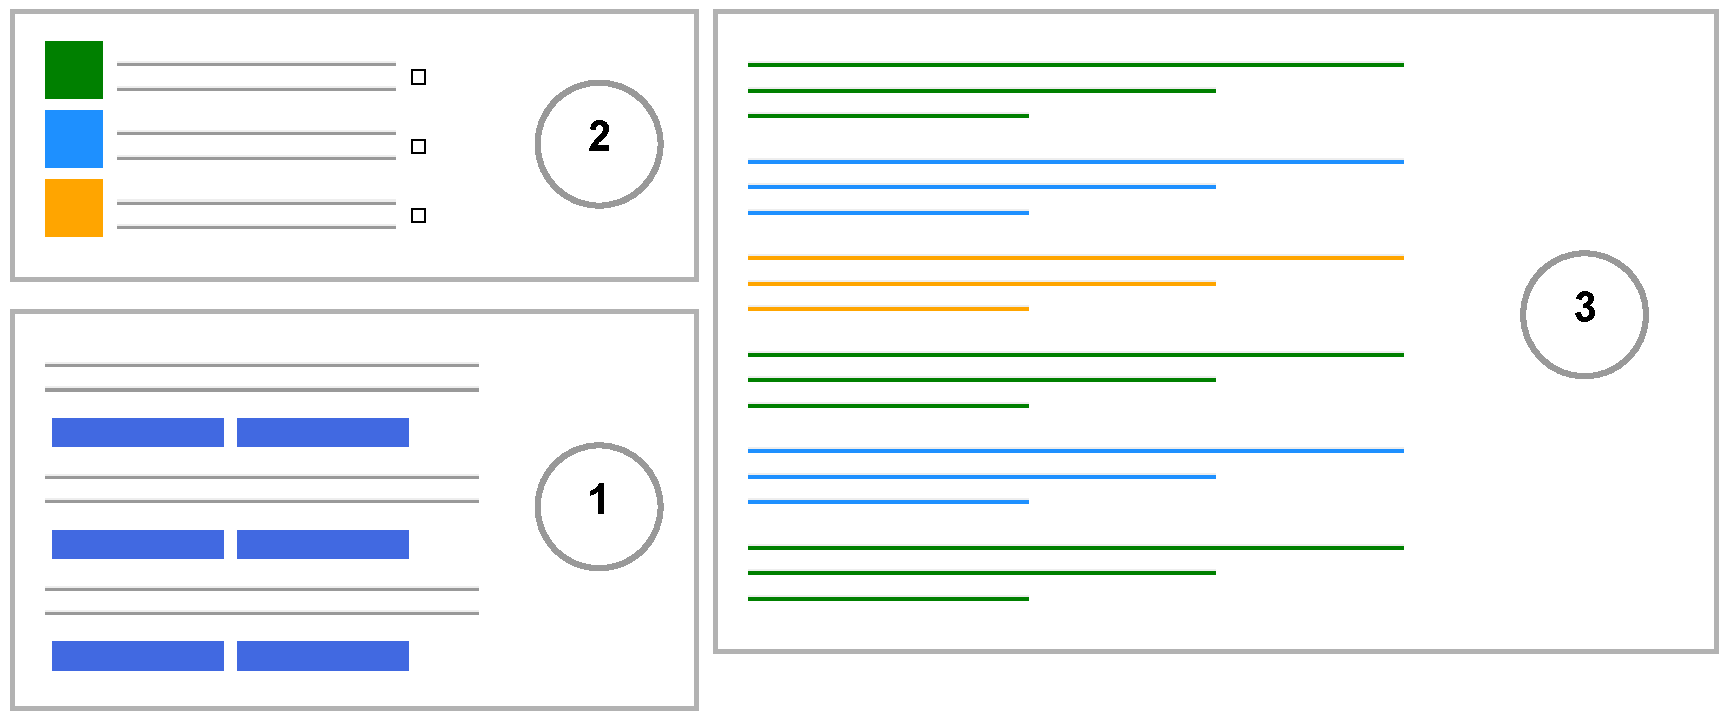
\includegraphics[width=0.7\textwidth]{img/collabIDEGeneral}
  \caption{CollabIDE tool}
  \label{fig:collabide}
\end{figure}

%%%%
\subsection{Experiment Setup}

Six developers were gathered for the Distributed Software Development experiment, then they were split into groups of two. Two groups would be using CollabIDE and the remaining group would be using Sublime Text in conjunction with git and github. The programming task for this experiment was to implement a set of common graph algorithms using only JavaScript. The participants were given a total of ninety minutes to accomplish this task. Each group was required to obtain their partner’s changes every fifteen minutes using their tools at hand.
In the Software Product Lines experiment, a different group of four developers was gathered. Two of them would be using CollabIDE and the other two would be using Eclipse in conjunction with git and github. In this case, the programming task was to implement a set of data structures with some basic functionality using JavaScript (CollabIDE) or Java (Eclipse). Each data structure also had to be a variant of a given base structure. These participants were also given ninety minutes to complete their task. In order to manage the different product variants, the participants were requested to use version control in each of their IDEs.


\authorcomment[missing]{NC}{Tools, exercise}
	

%%%%
\subsection{Results}

In this section we analyze the results of each experiment, specifically how each measure taken helps us tell if there was an increase in productivity.

\subsubsection{Experiment 1 Results}

First, in \fref{fig:resultsCollaborative} we show the results for each group and the background of each participant. Both groups that used CollabIDE achieved a higher completion rate (on average of 11 percent more tasks completed) than the control group (\fref{fig:completionCollaborative}). On top of that, they also spent significantly less time performing actions related to version control (an average of 33.2 less minutes) (\fref{fig:versionControlCollaborative}). The higher completion rate achieved by the groups that used CollabIDE can be attributed to the fact that the developers could spend more time coding as they didn’t have to invest much time in version control. It is clear why there is such a significant difference in time for both IDEs results. While the control group had to follow the common git workflow of committing, pushing, pulling changes and solving the possible conflicts that could arise, the CollabIDE groups could avoid this process altogether as CollabIDE’s features ensured that both team members always had each other latest changes without conflicts. Thus, the only action they needed to perform was creating a new version using the side menu of CollabIDE.

When analyzing the developers background, one factor that could have influenced the results is the fact that all of the participants that used CollabIDE had more experience in both Javascript and distributed development. Nevertheless, the experiment was designed in a way that only a basic knowledge of Javascript and data structures was required so the results were most likely not influenced by this.

\begin{figure}[htbp]
  \centering
  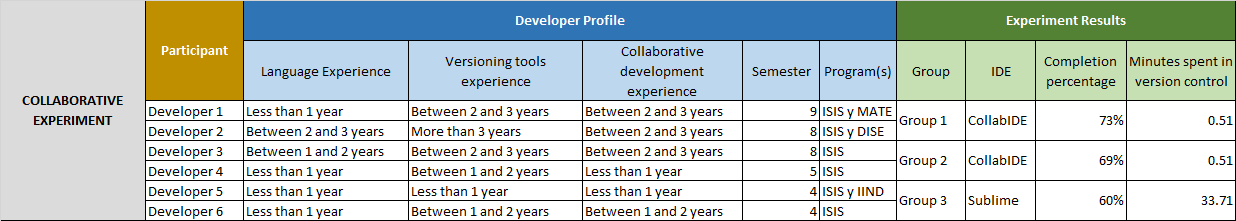
\includegraphics[width=1\textwidth]{img/resultsTableCollaborative}
  \caption{Distributed Development experiment results}
  \label{fig:resultsTableCollaborative}
\end{figure}

\begin{figure}[htbp]
  \centering
  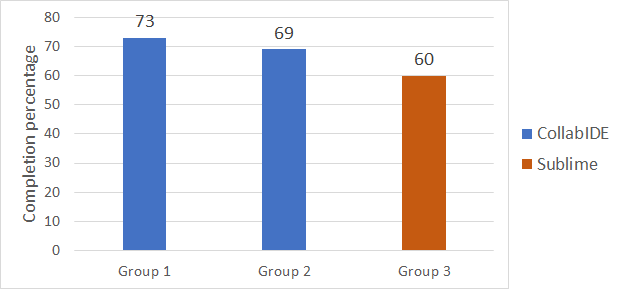
\includegraphics[width=0.8\textwidth]{img/completionCollaborative}
  \caption{Completion percentage graph for Distributed Development}
  \label{fig:completionCollaborative}
\end{figure}

\begin{figure}[htbp]
  \centering
  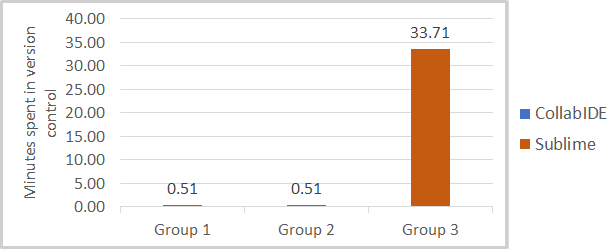
\includegraphics[width=0.8\textwidth]{img/versionControlCollaborative}
  \caption{Time spent in version control graph for Distributed Development}
  \label{fig:{img/versionControlCollaborative}}
\end{figure}

\subsubsection{Experiment 2 Results}

In \fref{fig:resultsTableProductLine} we show the results and background for each developer in the product line development experiment. Like the first experiment, the developers that employed CollabIDE obtained better results, but in this case, the difference between using one IDE versus using the other was not very significative. With CollabIDE, the developers finished on average 4 percent more tasks (\fref{fig:completionProductLine}) and spent 2.83 less minutes in version control than the developers using Eclipse (\fref{fig:versionControlProductLine}).The process of creating new product variants and their respective functionalities varied significantly in each IDE. With Eclipse and git, participants had to create a branch for each variant and then checkout between branches when they needed to work on a variant’s specific code. On the other hand, with CollabIDE, participants needed to first create a product version for each variant, then, for each variant create a new developer. This way the participants could take advantage of code highlighting, showing and hiding to easily distinguish which code fragments belonged to which variant. Thus, while Eclipse and Git makes variant creation straightforward, the process of switching between them isn’t as smooth. The contrary happens with CollabIDE where creating a variant is a longer process but switching between them is faster. According to this, it makes sense that in the results there wasn’t that big of a difference as there is a tradeoff when using one IDE versus the other. However, in real life contexts, projects usually take longer to complete and variant switching operations are more plentiful than variant creating ones. Therefore, in a real life context CollabIDE would provide better productivity for a development team.

When analyzing other factors that could have influenced the experiment, we found some with a potential impact on the results. First, the tasks needed to be implemented in differentes languages, the differences between languages could hadve lead to some developers having an easier time than others. Another outcome worth mentioning is that one of the developers had problems pushing his changes to github, and at the end of the experiment he only had one branch, meaning he lost the changes he made to various product variants. This occurrence helps reinforce our claim that even using version control systems can harm the productivity of a development team.   
\begin{figure}[htbp]
  \centering
  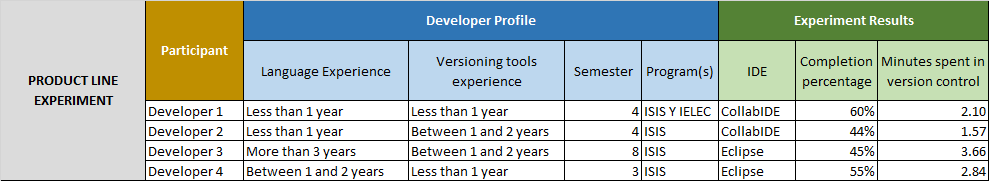
\includegraphics[width=1\textwidth]{img/resultsTableProductLine}
  \caption{Product Line Development experiment results}
  \label{fig:resultsTableProductLine}
\end{figure}

\begin{figure}[htbp]
  \centering
  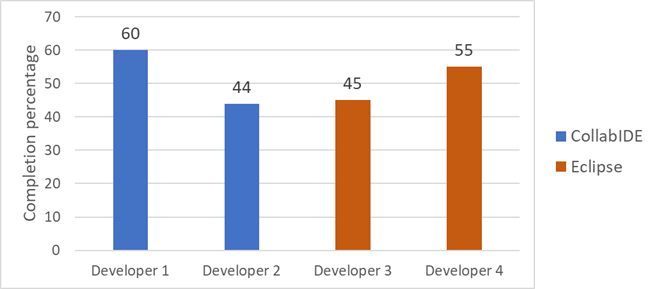
\includegraphics[width=0.8\textwidth]{img/completionProductLine}
  \caption{Completion percentage graph for Product Line Development}
  \label{fig:completionProductLine}
\end{figure}

\begin{figure}[htbp]
  \centering
  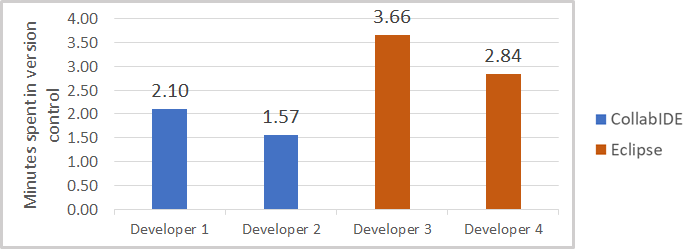
\includegraphics[width=0.8\textwidth]{img/versionControlProductLine}
  \caption{Time spent in version control graph for Product Line Development}
  \label{fig:versionControlProductLine}
\end{figure}

%%%%
\subsection{Threats to Validity}
In this section we discuss some aspects of the experiments that can put at risk the validity of the results discussed previously. The first one is that the subject sample size is small, having only one control group in the first experiment and two in the second. Small sample seizes can easily lead to bias [REF], and, in this case, the bias would be towards CollabIDE performing better. Another aspect that can be considered a threat is the low duration of each experiment. In real life contexts, software projects where version control systems are employed usually take months if not years to complete. Additionally, the time intervals between each version control operation are longer, whereas in the experiment they needed to be performed each fifteen minutes. These lower times could also lead to bias towards one of the IDEs, as the development workflow wasn’t completely accurate compared to one carried out in a real life context. 


\endinput

% $  Id: validation.tex  $
% !TEX root = main.tex


%%
\section{Related Work}
\label{sec:related}

Different tools exist for collaborative writing or coding.
In this section we discuss the features available in such tools and put them in perspective to CollabIDE.

\paragraph
{Collaborative writing platforms} like Google Docs and 
meetingwords\footnote{\url{http://meetingwords.com}} are not designed for code editing, 
however, they employ mechanics similar to those of CollabIDE’s. In Google Docs, changes made to a 
document are asynchronous and saved automatically. Contributions by collaborators are visible in real 
time by following user-specific markers. However,  changes are all merged into a single document as 
users edit. Nonetheless, color highlighting is used to highlight changes made by individual collaborators 
when reviewing a document’s history. Meetingwords provides similar features to those in Google Docs, 
with the additional feature of color highlighting for the editions each user contributes to the document. 
Such color highlighting served as inspiration for the same feature in CollabIDE. However, this is just a 
visual aid to see who contributed each part of the text, and cannot be manipulated as versions in 
CollabIDE.

\paragraph
{Distributed tools for code editing} targeting development productivity have also been 
explored.~\citet{ghorashi} present Jimbo, an IDE that allows developers to collaborate on a common 
project. Jimbo's most relevant features are synchronic and asynchronic collaboration, and user 
identification. The first one lets developers make changes without worrying about conflicts. The second 
one provides version management by allowing developers to follow specific fragments of code in a 
project to later receive notifications if said fragment received any modifications. This second feature may 
not be optimal on big projects where there are thousands of lines of code as it requires continuous user 
intervention, effectively creating an overhead that harms productivity. 
CodeBunk\footnote{\url{https://codebunk.com}}. is a cloud-based tool enabling playback. Playback 
saves the history of all changes made in an instance of the code editor. Users can playback these 
changes, showing each one in the order they were made. This feature reduces conflicts and improve 
awareness in a project. Similar to Jimbo, an overhead is introduced as developers need to interrupt 
their workflow and sit through a history’s playback to identify possible conflicts and changes made by 
others. If an history gets long enough, the interruption times also get longer, and more time is needed 
to get back into the coding workflow.

In CollabIDE, both of these overhead problems are avoided by providing passive aids to developers for 
(automatic) code versioning, and identifying distinct user’s contributions (code highlighting). This way 
developers can focus on writing code rather than on performing additional actions.


\endinput


% $  Id: conclusion.tex  $
% !TEX root = main.tex

%%
\section{Conclusion}
\label{sec:conclusion}

CollabIDE is a development environment prototype for distributed teams, incorporating automated versioning and enabling the generation of multiple software products according to the code's versions base.

CollabIDE is developed with the goal of increasing the productivity of software development teams by reducing the time developers must dedicate to tasks other than coding. CollabIDE specifically targets the versioning and product variant deployment tasks of the software development process. CollabIDE is based on \ac{COP} to tackle both tasks. Contextual situations in which the development task take place (\eg user, time, code extract of the modification) are defined as contexts adaptations, which can be use directly to represent and define the versions of the system. Extraction, definition, and usage of such contexts/versions takes place autonomously, so developers need no to be distracted by these activities. 
\ac{COP} enables a flexible composition of software systems while they execute. Using this feature it is possible to compose different versions as part of a fully working program variant. Composition of such variants requires developers to select which of the contexts they want to use. Available contexts in the project are accessible to developers within the tool itself, in order to minimize the disruption and time spent in generating the variants.

The validation evidences that CollabIDE effectively makes a step forward towards reducing the overhead of dealing with version control systems and product variant generation, when working in a distributed software development team.
Although the scale of the experiment is small, it already shows the potential that an approach like 
CollabIDE has. Thanks to the flexibility of the technology used to create CollabIDE.......

As future work, we plan to conduct a more extensive case study to evaluate the relevance of CollabIDE in larger development teams. Additionally, we see the value of the tool for code reviews, therefore we want to extend CollabIDE with code productivity metrics (\eg Lines of Code, code clones) and analysis facilities~\cite{lienhard12}. Such extension would enable code reviewers to better evaluate the productivity of particular developers. CollabIDE, can be particularly useful in academic/teaching environments to quickly differentiate how much a particular student participated in an assignment, when did the majority of the work took place.

\endinput



%
%\balancecolumns

%\printbibliography
\bibliographystyle{splncs03}
\bibliography{local,bib/compsci,bib/general,bib/learning,bib/collabide}  


\end{document}

